\documentclass{article}
\usepackage{tikz}
\usetikzlibrary{fit, positioning}

\begin{document}

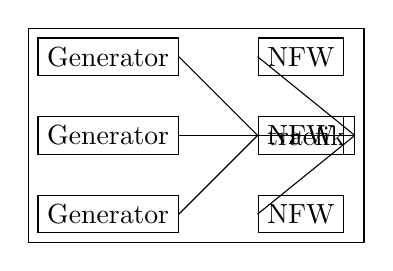
\begin{tikzpicture}

\node (base) at (0, 0) {};

% generators
\foreach \m in {1, 2, 3} {
    \node[draw, below = of base] (generator-\m) at (0, \m) {Generator};
}

% NFW calculators
\foreach \m in {1, 2, 3} {
    \node[draw, right = of generator-\m] (NFW-\m) {NFW};
}

% generatortraefik
\node[draw, right = of generator-2] (generatortraefik) {traefik};

% connect the generators with the generatortraefik
\foreach \l in {1, 2, 3} {
    \draw (generator-\l.east) -- (generatortraefik.west) {};
}

% connect the generatortraefik with the NFW nodes
\foreach \l in {1, 2, 3} {
    \draw (generatortraefik.east) -- (NFW-\l.west) {};
}

\node[draw, fit=
    (generator-1)
    (generator-2)
    (generator-3)
    (generatortraefik)
    (NFW-1)
    (NFW-2)
    (NFW-3)
] (boundary) {};

\end{tikzpicture}

\end{document}
